\chapter{Literature review}\label{sec:literature}
\section{Preliminaries on robo-advisors}

The inception of robo-advisors dates back to the early 2000s when the first online investment platforms, such as Betterment and Wealthfront, came to the fore. These platforms leveraged algorithms to determine asset allocation and rebalancing strategies, providing automated investment advice and portfolio management services to individual investors at a low cost. With the advancement of technology, traditional financial institutions started offering robo-advisory services by developing their own platforms or collaborating with existing FinTech firms.

The financial crisis of 2008 was a turning point in investment management. The crisis led to a loss of trust in traditional financial institutions, prompting investors to explore alternative investment strategies. This environment facilitated the emergence of robo-advising, which offers investors an automated investment platform that uses quantitative algorithms to manage their portfolios \cite{capponi2022personalized}. This platform is easily accessible to clients online, allowing investors to create and manage their portfolios. The robo-advisor analyzes the investor's risk tolerance, investment goals, and financial situation using algorithms to develop a personalized investment plan for the investor \cite{beketov2018robo}. The platform then uses these algorithms to execute trades and manage the investor's portfolio on an ongoing basis.

The robo-advisory industry is relatively new, but it has grown rapidly since its inception in response to the increasing demand from investors for more transparent and low-cost investment services. Using robo-advisors provides several benefits to financial institutions and investors alike. One of the main benefits of using robo-advisors is that they save on fixed costs for financial institutions. The traditional model of investment advisory services involves human advisors who charge high fees for their services. In contrast, robo-advisors offer similar investment advice at a fraction of the cost, making it more accessible and affordable to a broader range of investors \cite{beketov2018robo}.

Furthermore, robo-advisors provide systematic and transparent advice to a new generation of clients \cite{alsabah2021robo,beketov2018robo}. They use algorithms to create personalized investment plans tailored to the investor's risk tolerance and financial situation. This approach provides investors with more transparent and objective advice than traditional investment advisory services, which can be influenced by the advisor's biases.

The robo-advisory industry has grown rapidly since its inception, and this trend is expected to continue in the future. As more investors turn to digital investment platforms, the number of robo-advisors on the market continues to increase, and established players are expanding their offerings to remain competitive. Many robo-advisors are also becoming more sophisticated, offering a wider range of investment options such as socially responsible investing and alternative investments. Assets under management in the robo-advisory segment are projected to reach US\$2.76 trillion in 2023 \cite{statista2023}. The growth of the industry is being driven by several factors, including increased investor demand for low-cost and transparent investment services and the proliferation of new technology that makes robo-advisors more accessible to a broader range of investors. 

\section{Pipeline of a robo-advisor}
\begin{figure}
    \centering
    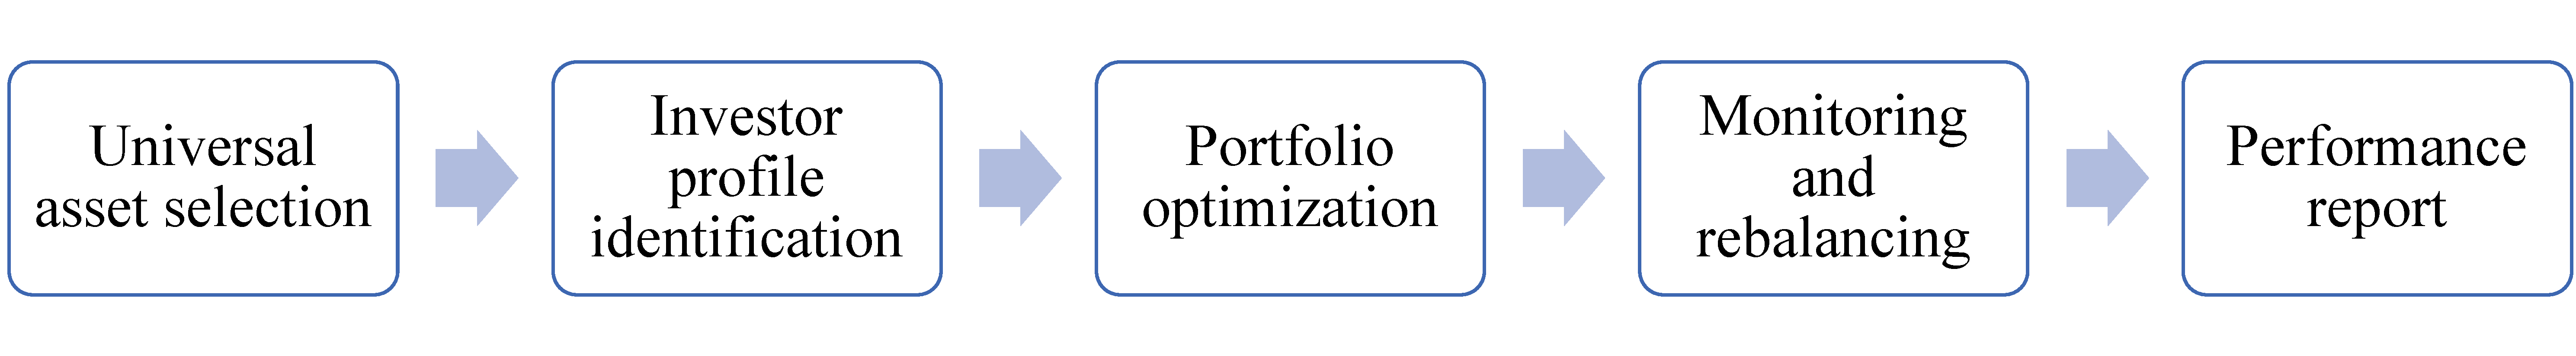
\includegraphics[width=1\textwidth]{imgs/pipeline.pdf}
    \caption{Pipeline of a typical robo-advisor \protect\cite{beketov2018robo}.}
    \label{fig:pipeline}
\end{figure}
As per \cite{beketov2018robo}, a typical robo-advisor has the following blocks, as shown in Figure \ref{fig:pipeline}.\begin{enumerate}
    \item \textbf{Universal asset selection.} This block involves providing a set of investment instruments that the robo-advisor can select from based on their corresponding risk and return information. The set of instruments is usually predetermined and provided by human financial advisors to the robo-advisor to choose from, rather than being chosen by the advisor itself. This approach allows for greater consistency in investment options across clients and helps to ensure that all clients have access to the same investment opportunities.

    \item \textbf{Investor profile identification.} In this block, the robo-advisor models and infers the client's risk profile and investment preferences. This can be done through various means, such as questionnaires \cite{tertilt2018advise}, portfolio choices \cite{alsabah2021robo}, or client interactions \cite{capponi2022personalized}. The goal is to understand the client's risk tolerance, investment goals, and other factors that may impact their investment decisions. By understanding the client's profile, the robo-advisor can provide personalized investment advice that is tailored to the client's specific needs.

    \item \textbf{Portfolio optimization.} This block involves the optimization of the client's portfolio selection based on their risk profile and investment preferences. The robo-advisor uses algorithms to determine the optimal investment mix for the client based on factors such as risk tolerance, expected return, and investment horizon. Robo-advisors may use different optimization objectives to perform optimal asset allocation, such as to maximize mean-variance objective \cite{capponi2022personalized,alsabah2021robo,wang2021robo} or to minimize risk with a constraint on the target mean return \cite{wang2020continuous}. This allows for the efficient management of client portfolios and can help to maximize returns while minimizing risk.

    \item \textbf{Monitoring and rebalancing.} The robo-advisor must continually monitor the performance of the selected investment policy and intervene when necessary. This may involve re-estimating the client's risk profile, adjusting the investment mix, or rebalancing the portfolio to ensure that it remains aligned with the client's investment goals. The robo-advisor may re-estimate the user’s risk profile because (i) it finds its previous estimation not accurate; (ii) the client’s risk profile may change from time to time. By providing ongoing monitoring and management, the robo-advisor can help clients stay on track to achieve their investment objectives. 

    \item \textbf{Performance report.} Finally, the robo-advisor should provide performance reports to clients to keep them informed about the performance of their investments, just like their human counterparts. This may include details on investment returns, fees, and other relevant information. By providing clients with regular updates, the robo-advisor can help to build trust and confidence in the investment management process.
\end{enumerate}

In this report, we have a particular focus on the second, third and fourth blocks of a robo-advisor's pipeline -- investor profile identification, portfolio optimization and monitoring and rebalancing. We aim to design a robo-advisor that models and estimates the risk profile of a client, exploits its estimation to optimize portfolio, and re-estimates the risk profile and rebalances the portfolio when it finds necessary, through client interactions or actively asking client for intervening.

\section{Existing robo-advisors and a taxonomy of them}
Not only have robo-advisors drawn an emerging amount of attention in financial institutions and investors, but they have grown more and more popular in the quantitative finance research community as well. In this section, we study a few existing robo-advising models in the literature and give a taxonomy of robo-advisors based on their optimization goal, client input to the robo-advisor and the robo-advisor's interaction model. We focus on robo-advisors from the works of \citeA{capponi2022personalized}, \citeA{alsabah2021robo}, \citeA{wang2020continuous} and \citeA{wang2021robo}.

\begin{table}[t]
    \centering
    \begin{tabular}{p{1.5cm}p{2.5cm}p{4cm}p{5.5cm}}
    \toprule
        \textsc{Model} & \textsc{Optimization Goal} &\textsc{Client Input} & \textsc{Interaction Model}\\\midrule
         \citeA{wang2020continuous} & Risk minimization given target return. Not personalized. & Target return value. & No interaction. \\\hline
         \citeA{wang2021robo} & Mean-variance objective with risk aversion. & Historical actions of the client where risk aversion is to be learnt through IRL. & No interactions.\\\hline
         \citeA{alsabah2021robo} & Mean-variance objective with risk aversion. & Historical and interactive actions of the client. Due to the bijection between risk aversion to action, this is equivalent to numerical risk aversion values.& Interactions with the client are initiated by the robo-advisor to receive updated risk aversion parameters with penalty on each interaction, resulting in exploration-exploitation trade-off.\\\hline
         \citeA{capponi2022personalized} & Mean-variance objective with risk aversion. & Interactive behaviorally biased risk aversion parameters communicated by the client.& Interactions with the client are determined by a fixed interaction schedule and there's no explicit penalty on interactions. However, the behavioral bias at interaction times lead to trade-off between more interactions versus less bias.\\
         \bottomrule
    \end{tabular}
    \caption{A taxomony of selected robo-advisors in the literature.}
    \label{tab:taxomony}
\end{table}

We classify any robo-advisor based on three dimensions.\begin{enumerate}
    \item \textbf{Optimization goal.} Regardless of what and how a robo-advisor may communicate with its client, it may take different optimization goals for portfolio selection. This is the core component of the third block, portfolio optimization, of a robo-advisor's pipeline as shown in Figure \ref{fig:pipeline}. Since optimization goal is of particular importance to a robo-advisor, we first categorize robo-advisors based on their optimization goals. In general, there are two types of optimization goals:\begin{enumerate}
        \item Personalizaed optimization goals. Robo-advisors whose optimization goals are determined by the client's risk profile and investment goals provide personalized investment advisory tailored to the client's needs. Robo-advisors with personalized optimization goals consider the risk aversion of different clients and make investment decisions based on it. Assuming the client's risk aversion is $\gamma$, then the most common optimization goal is to maximize the mean-variance objective function $\E[X]-\gamma/2\Var[X]$ where $X$ is the client's wealth. In this setting, since the robo-advisor cannot always have complete information on the client's varying risk aversion over time (otherwise it would be equivalant to the client investing on herself), the advisor must estimate and update this value by modelling and interactions with the client. \citeA{capponi2022personalized}, \citeA{alsabah2021robo}  and \citeA{wang2021robo} can all be categorized as robo-advisors with personalized optimization goals.
        \item Non-personalized optimization goals. A simplified method is to model the mean variance portfolio selection problem as a variance minimization process with fixed target return. In this setting, the advisor only needs to ask the client for the target return, and then selects the portfolio with the minimum risk. \citeA{wang2020continuous} can be categorized here where they use a reinforcement learning framework to solve the variance minimization problem. This is \textbf{not} personalized.
    \end{enumerate}
    \item \textbf{Communicated client input.} In this dimension, we categorize robo-advisors based on \textit{what} (i.e., the content) the client communicates with the advisor into two classes.\begin{enumerate}
        \item The robo-advisor can directly obtain the required \textit{parameter} (for example, client's risk aversion) from the client. This is a high level abstraction since the actual process of this may be more complicated (since the client is unable to give a numerical value for her risk aversion, but such value can be obtained from a questionnaire), which is out of our concern. Note that it is preferable to also consider and model the bias of this communicated risk aversion, as in \citeA{capponi2022personalized} where they consider the behavioral bias of the client at interaction times due to trend-chasing mindset. We also classify \citeA{alsabah2021robo} here because although the client input to the robo-advisor is her investment actions, they assume the function from risk aversion $\gamma$ to the client's action is bijective and invertible, hence, it is equivalent to the case where the client directly communicates her risk aversion to the robo-advisor. In \citeA{alsabah2021robo}, they do not consider behavioral bias in the communicated risk aversion.
        \item The robo-advisor may be not able to obtain the required parameter such as risk aversion, but the robo-advisor may be able to observe client's \textit{strategies and actions} instead. Such strategies usually refer to client's asset allocation decisions made in a market with complete information. The behavior observed by the robo-advisor may be historical, i.e., client's actions before the robo-advising process as a reference, or interactive, i.e., the robo-advisor observes or asks for the client's decisions on an ongoing basis. In this case, the problem can be modelled as a inverse reinforcement learning problem \cite{ng2000algorithms} where one can only observe the client's actions to the environment and infer the client's internal parameters to be used for robo-advised investment later. \citeA{wang2021robo} propose a deep reinforcement learning algorithm to infer the risk preference of the client from historical client's asset allocations.
    \end{enumerate}
    \item \textbf{Interaction model.} At last, robo-advisors can also be categorized based on their interaction models. First, they can be classified into those with and without interactions with the client.\begin{enumerate}
        \item Robo-advisors without interactions with the client obtain all the information required from the client in a single information exchange. The robo-advisor may obtain the client's target risk or risk aversion through direct communication of numerical values or can estimate the required parameters from historical allocations of the client. The robo-advisor in \citeA{wang2020continuous} receives a single target return value from the client to perform risk minimization with constraint on target return value. \citeA{wang2021robo} let the robo-advisor to receive historical asset allocations of the client to infer the client's risk aversion. Both do not involve interactive communications during the robo-advising process.
        \item There are also robo-advisors that allow interactions with the client during the robo-advising process. In this case,  the robo-advisor may interact with the client (explore for better estimation of the risk aversion parameter), and optimize based on the information received (exploit the current belief of the risk aversion to make decisions). Such interactions may come with an opportunity cost (i.e., a penalty), naturally leading to an exploration-exploitation trade-off where the robo-advisor cannot choose to interact with client all the time for perfect estimation of client's risk aversion. This is the case in \citeA{alsabah2021robo}. \citeA{capponi2022personalized} take an alternative approach where there is no explicit penalty to the reward function on interactions. However, as they also consider the client's behavioral bias that is only activated at interaction times due to trend-chasing mindset, there is an implicit penalty for too many interactions and hence leading to a trade-off between better estimations and less behavioral bias. This is discussed in much detail in Section \ref{sec:personalize}.
    \end{enumerate}
\end{enumerate}

Table \ref{tab:taxomony} concludes our taxonomy for robo-advisors and categorizes each of the models we study into one of the categories in each dimension.
